\chapter{Realimentación Negativa en Amplificadores}\label{realimentacion}

\hspace{10pt} En este capítulo se presentan herramientas para el análisis y diseño de amplificadores realimentados utilizando LTSpice, sustentadas en los desarrollos presentados en  la bibliografía básica del tema \cite{gray95} \cite{sedra99}. 

En la figura \ref{real1} se muestra la estructura básica de un
amplificador con realimentación. En ella se presentan señales
genéricas (X), que pueden ser tensiones o corrientes según
el tipo de amplificador que se diseñe. La señal $X_o$ representa la
salida mientras que la señal $X_i$ corresponde a la entrada. La
señal $X_f=\textsf{f} X_o$ es una muestra de la salida, la señal $X_e$ es la
resta $X_i-X_f$ y la señal de salida $X_o=a X_e$. De estas
expresiones se deduce la expresión de la ganancia realimentada $A$:


\begin{equation}\label{ecreal1}
A=\frac {\displaystyle X_o}{\displaystyle X_i}=\frac{ \displaystyle a}{\displaystyle 1+a
 \textsf{f}}
\end{equation}


\begin{figure}
    \centering
    
\includegraphics[width=0.5\linewidth]{figuras/real1.png}
    \caption{Estructura general de un amplificador realimentado.}
    \label{real1}
\end{figure}

El signo del restador determina que la realimentación sea negativa.
El esquema ideal mostrado en la figura \ref{real1} responde a las
siguientes características:

\begin{itemize}
    \item Se denomina ganancia de lazo cerrado, o realimentada, $A$ a la
    expresión de la ecuación \ref{ecreal1}.
    \item La transferencia $a=\frac{\displaystyle X_o}{\displaystyle
    X_e}$ es la ganancia sin realimentar (con $\textsf{f}=0$), en el esquema
    ideal esta ganancia es unilateral en sentido directo.
    \item La señal $X_e=X_i-X_f$, se denomina señal de error.
    \item La transferencia $\textsf{f}=\frac{\displaystyle X_f}{\displaystyle
    X_o}$ es la de la red de realimentación. Idealmente
    debe ser unilateral en sentido inverso.
    \item Se define $T=a\textsf{f}$ y se la denomina ganancia de lazo.
    \item En un sistema ideal los efectos de la carga a la salida y
    de la fuente en la entrada son nulos.
\end{itemize}

Bajo estas condiciones se puede expresar la ecuación \ref{ecreal1}
del siguiente modo:

\begin{equation}
\frac {\displaystyle X_o}{\displaystyle X_i}=\frac{ \displaystyle a}{\displaystyle
1+T}
\end{equation}

En una primera aplicación si $T\gg 1 \Rightarrow A \simeq
\frac{\displaystyle 1}{\displaystyle \textsf{f}}$, es decir que la ganancia
$A$ estará determinada sólo por $\textsf{f}$ (independiente de $a$) y si
$\mid \textsf{f}\mid < 1$, habrá amplificación.

De las expresiones anteriores se puede también derivar:
\medskip
\medskip
\medskip
\medskip
\begin{equation}
\frac {\displaystyle X_e}{\displaystyle X_i}=\frac{ \displaystyle 1}{\displaystyle
1+T} \qquad , \frac {\displaystyle X_f}{\displaystyle X_i}=\frac{
\displaystyle T}{\displaystyle 1+T}
\end{equation}
\medskip
\medskip
\medskip
\medskip
\section{Amplificadores de tensión. Configuración Serie-Paralelo}

\hspace{10pt} Los amplificadores de tensión son esencialmente fuentes de tensión
controladas por tensión, es necesario que la impedancia de entrada
sea alta y la impedancia de salida sea baja para que las
resistencias de fuente y de carga no influyan apreciablemente en la
transferencia. Como lo que se busca es estabilizar la transferencia
de tensión se requiere un muestreo de tensión en paralelo a la
salida y una realimentación de una tensión proporcional en serie a
la entrada. En la figura \ref{real2} se muestra el esquema ideal de
una realimentación serie-paralelo para un amplificador de tensión, es decir se considera que la impedancia del generador de entrada tiende a $0$ , que la impedancia de la carga tiende a $ \infty$ y que la realimentación está implementada como una fuente de tensión controlada por la tensión de salida $V_o$ ($E_2$) puesta en serie con la entrada con una transferencia de $0.0909$.

\begin{figure}[h]
	\centering
	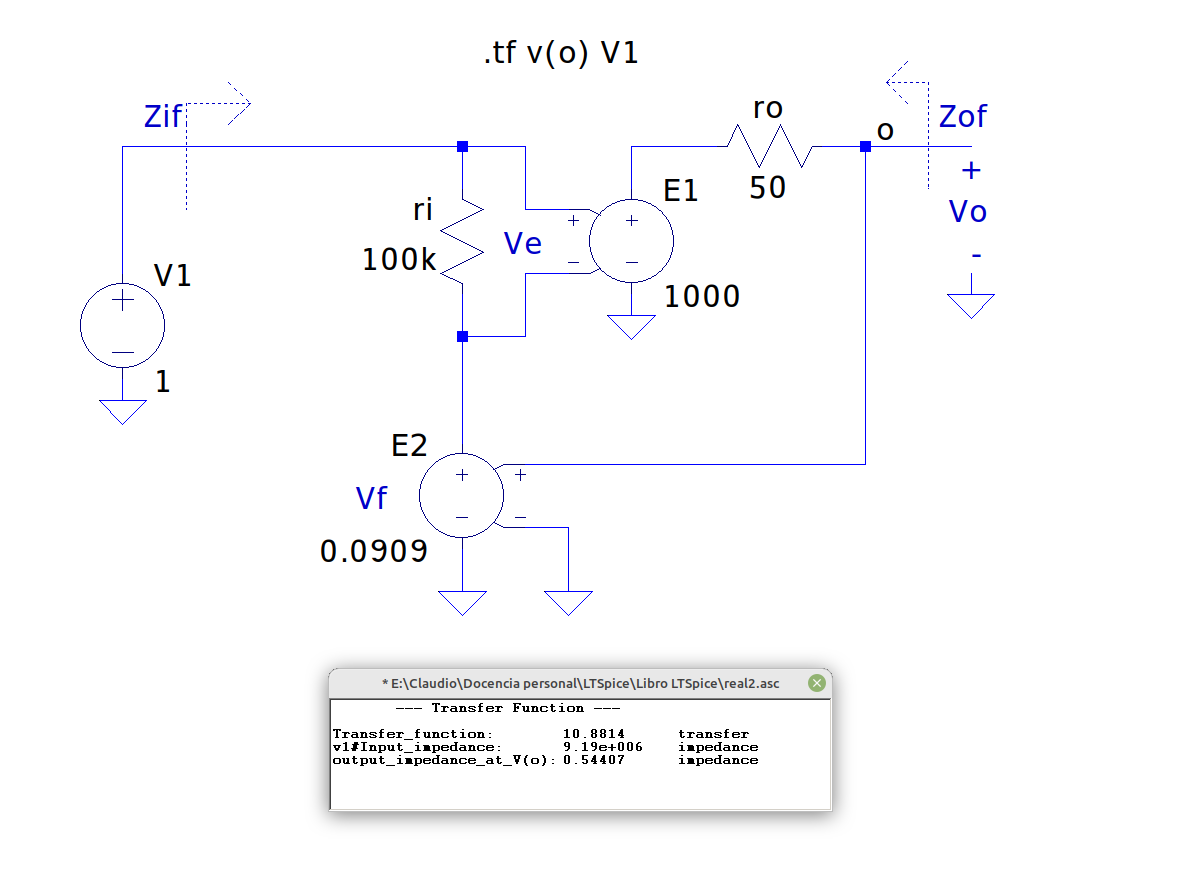
\includegraphics[width=1.0\linewidth]{figuras/real2x.png}
	\caption{Esquema ideal de una configuración Serie-Paralelo.}
	\label{real2}
\end{figure}


En dicha figura se aprecia una correspondencia completa con el
esquema ideal de la figura \ref{real1}; es decir $V_1$, $V_e$, $V_f$
y $V_o$ corresponden a $X_i$, $X_e$, $X_f$ y $X_o$ ,la ganancia
de valor $1000$ de la fuente de tensión controlada $E_1$ a la ganancia sin realimentar $a$ (ganancia con $\textsf{f}=0$) y la ganancia de valor $0.0909$ de la fuente de tensión controlada $E_2$ a la transferencia de la red de realimentación $\textsf{f}$, por lo que la ganancia realimentada será $A=\frac{\displaystyle V_o}{\displaystyle V_1}=\frac{\displaystyle a}{\displaystyle 1+a\textsf{f}}=\frac{\displaystyle 1000}{\displaystyle 1+1000 \times 0.0909}=10.88139 $ . Si se calcula la impedancia de entrada $Z_{if}$ que ''ve`` el generador $V_1$ se llega a: $Z_{if}=r_i(1+a\textsf{f})=9.19M\Omega$, siendo $r_i=100K\Omega$ la impedancia de entrada del amplificador sin realimentar ($\textsf{f}=0$) y $(1+a\textsf{f})$ la ganancia de lazo mas uno. Por otro lado la impedancia de salida vista desde $V_o$ se calcula anulando la tensión de entrada $V_1$, dando como resultado: $Z_{of}=\frac{\displaystyle r_o}{(\displaystyle 1+a\textsf{f})}=0.554069\Omega$, siendo $r_o$ la impedancia de salida sin realimentar ($\textsf{f}=0$). Estos resultados teóricos se verifican con los resultados de la simulación utilizando la directiva \textit{.tf v(o) v1}, mostrados en la parte inferior de la figura \ref{real2}





Un caso más cercano al real es el mostrado en la figura \ref{real3}, al amplificador de tensión básico se lo realimenta con una red resistiva $R_1$ y $R_2$, se lo carga con una $R_L$ y el generador de entrada tiene un resistencia $R_g$. 

\begin{figure}[h]
	\centering
	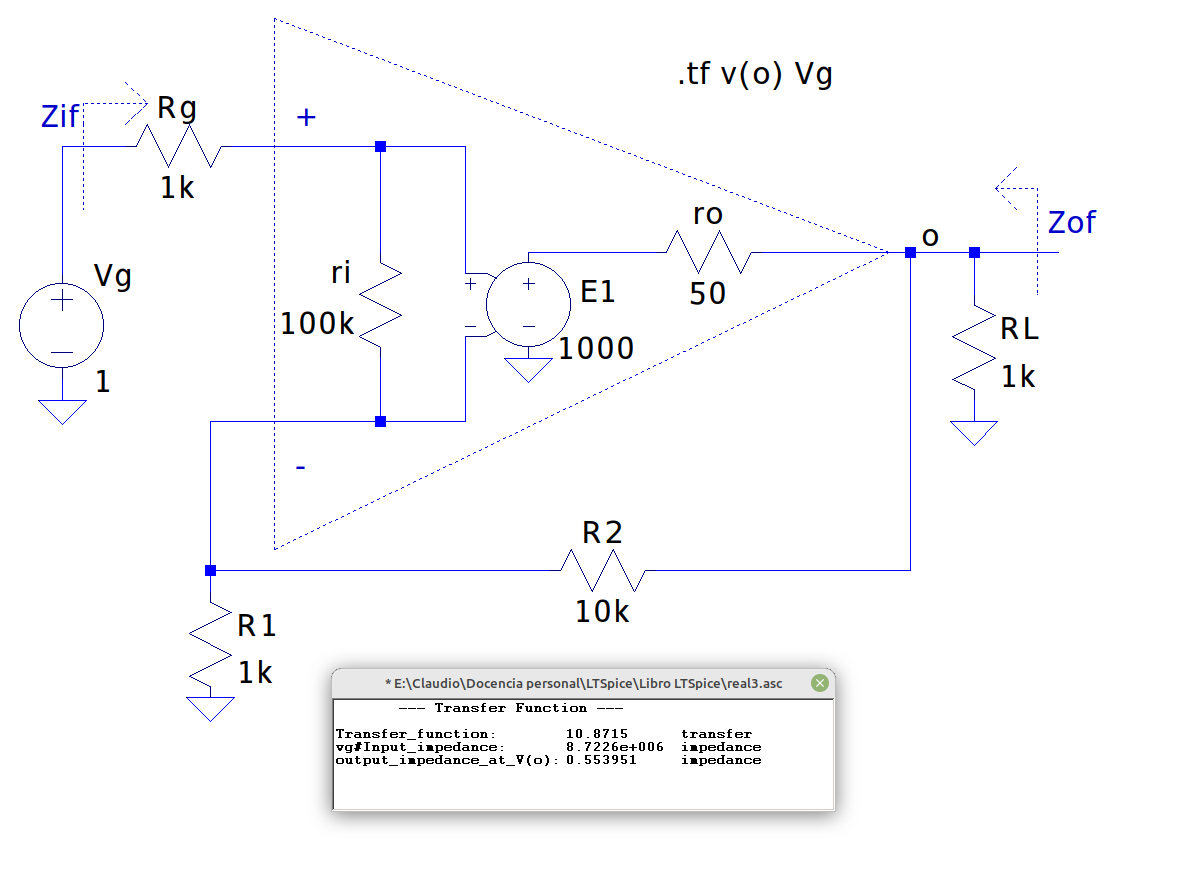
\includegraphics[width=1.0\linewidth]{figuras/real3x.png}
	\caption{Configuración Serie-Paralelo. Esquema real.}
	\label{real3}
\end{figure}

Si se reemplaza la red de realimentación formada por $R_1$ y $R_2$ por su red equivalente en parámetros $h$ se obtiene el circuito de la figura \ref{real4}, con $h_{11}=R_1||R_2$, $h_{22}=\frac{\displaystyle 1}{\displaystyle R_1+R_2}$ y $h_{12}=\frac{\displaystyle R_1}{\displaystyle R_1+R_2}$, suponiendo a la tranferencia directa de la red de realimentación (parámetro $h_{21}\approx 0$) despreciable frente a la transferencia directa de la red de amplificación. 

Los resultados de las simulaciones de los circuitos de las figuras \ref{real3} y \ref{real4} son equivalentes con la única aproximación ya mencionada. 

Si en la figura \ref{real4} se anula sólo el parámetro de realimentación $h_{12}=\textsf{f}=0$, se obtiene el circuito sin realimentar con los efectos de carga incluidos, como establece la teoría clásica de realimentación \cite{gray95}. En la figura \ref{real5} se muestra el resultado de la simulación \textit{.tf v(o) vq} con $\textsf{f}=0$, en esta situación se obtienen la ganancia de tensión sin realimentar $a_v=930.512$, la impedancia de entrada sin realimentar $Z_{io}=101909\Omega$ y la impedancia de salida sin realimentar $Z_{oo}=47.4139\Omega$. Si se considera que $\textsf{f}=0.909$ el resultado teórico mostrado a continuación coincide con el simulado en la figura \ref{real4}:

\medskip
\medskip
\medskip

\begin{equation}
\begin{split}
A_v &=\frac{\displaystyle a_v}{\displaystyle 1+a_v\textsf{f}}=10.87256 \\
Z_{if} &= Z_{io}(1+a_v\textsf{f})=8.72173M\Omega \\
Z_{of} &= \frac{\displaystyle Z_{oo}}{\displaystyle 1+a_v\textsf{f}}=0.5540\Omega
\end{split}
\end{equation} 

\medskip
\medskip
\medskip



\begin{figure}
    \centering
    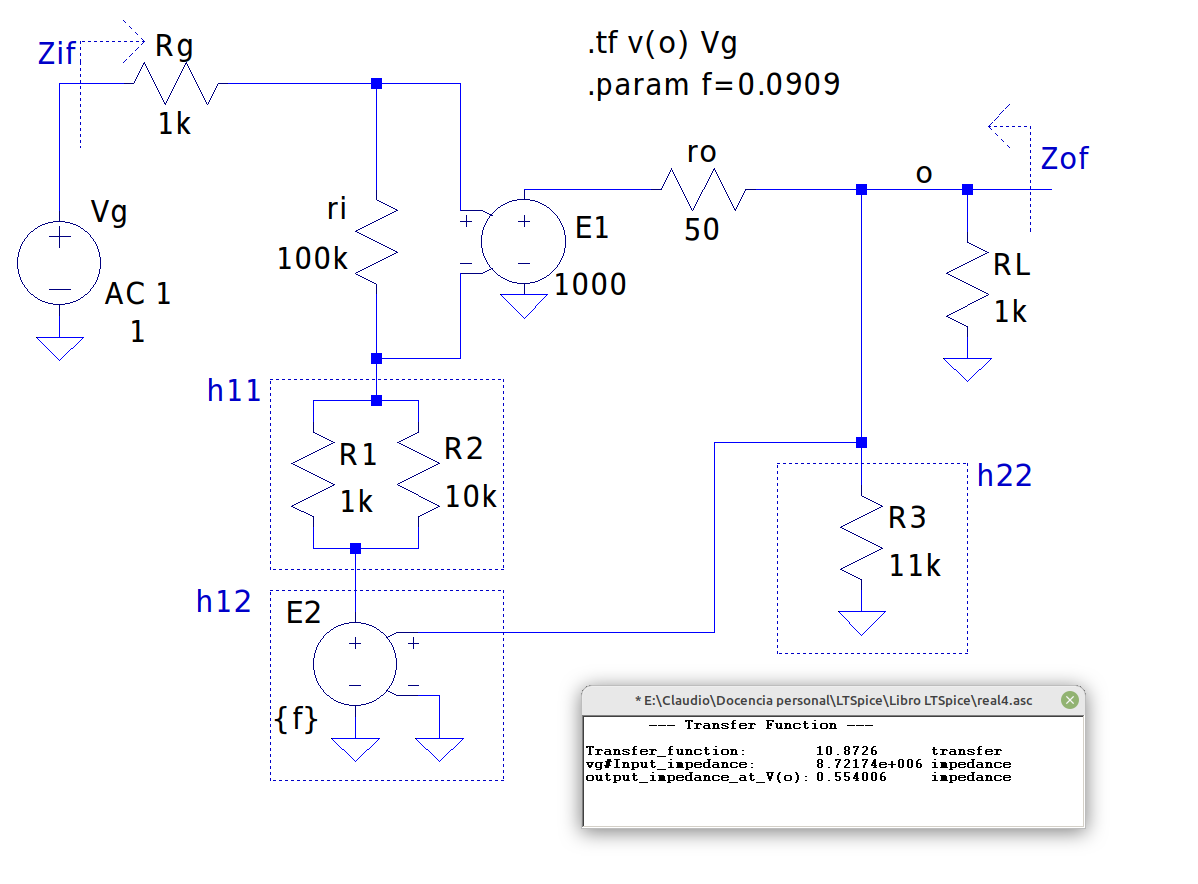
\includegraphics[width=1.0\linewidth]{figuras/real4x.png}
    \caption{Configuración Serie-Paralelo. Reemplazo de las red de realimentación por su equivalente en parámetros h.}
    \label{real4}
\end{figure}

\begin{figure}
    \centering
    
\includegraphics[width=0.5\linewidth]{figuras/real5.png}
    \caption{Configuración Serie-Paralelo. Transferencia sin realimentar con efectos de carga incluidos.}
    \label{real5}
\end{figure}

\section{Amplificadores de corriente. Configuración Paralelo-Serie}

\hspace{10pt} Los amplificadores de corriente son fuentes de corriente
controladas por corriente, es necesario que la impedancia de entrada
sea baja y la impedancia de salida sea alta para que las
resistencias de fuente y de carga no influyan apreciablemente en la
transferencia. Como lo que se busca es estabilizar la transferencia
de corriente se requiere un muestreo de corriente en serie a la 
salida y una realimentación de una corriente proporcional en paralelo a
la fuente de entrada. Siguiendo los lineamientos generales de la teoría clásica de realimentación \cite{gray95} para el caso de esta configuración se puede resumir que: 

\begin{itemize}
	\item El generador de entrada es de corriente, $i_g$.
	\item La salida a controlar es una corriente, $i_o$.
	\item La red de realimentación deberá reemplazarse por su equivalente en parámetros $[g]$, considerando despreciable el parámetro de transferencia directa $g_{21}$.
	\item La ganancia de corriente sin realimentar $(a_i)$ debe ser la obtenida anulando el parámetro de realimentación $\textsf{f}=g_{12}$. Es decir con la inclusión de los efectos de carga $g_{11}$ y $g_{22}$.
	\item La ganancia realimentada será: $A_i=\frac{\displaystyle i_g}{\displaystyle i_o}=\frac{\displaystyle a_i}{\displaystyle 1+a_i\textsf{f}}$ 
	\item La impedancia de entrada realimentada que "ve" el generador $i_g$ es: $Z_{if}=\frac{\displaystyle Z_{io}}{\displaystyle 1+a_i\textsf{f}}$, siendo $Z_{io}$ la impedancia de entrada sin realimentar con $\textsf{f}=0$ incluyendo los efectos de carga.
	\item La impedancia de salida realimentada que presenta el circuito en serie con la corriente $i_o$ es: $Z_{of}=Z_{oo}(1+a_i\textsf{f})$, siendo $Z_{oo}$ la impedancia de salida sin realimentar con $\textsf{f}=0$ incluyendo los efectos de carga.
\end{itemize} 


El circuito de la figura \ref{real6} es un amplificador de corriente, siendo la red de realimentación la formada por las resistencias $R_3$ y $R_4$, que sensan la corriente $i_o$ y una proporción de dicha corriente es realimentada en paralelo a la entrada a través de la corriente $i_f$.

\begin{figure}[h]
	\centering
	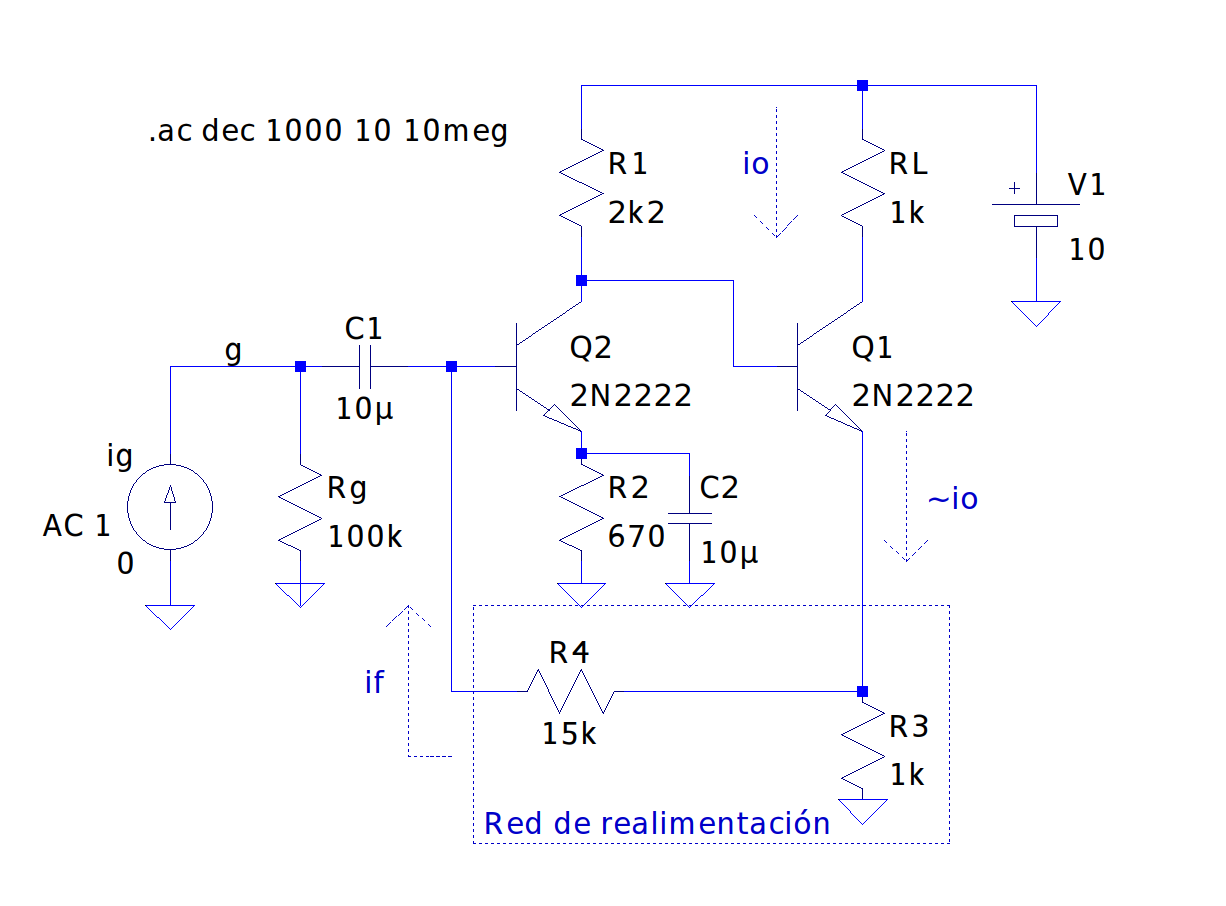
\includegraphics[width=1.0\linewidth]{figuras/real6x.png}
	\caption{Amplificador realimentado de corriente.}
	\label{real6}
\end{figure}

 En este circuito no se puede aplicar directamente la directiva \textit{.tf} para hallar la transferencia y las impedancias  por tratarse de un análisis de continua y la presencia de los capacitores $C_1$ y $C_2$ darían resultados erróneos. Para utilizarla se debería hallar primero el punto de operación de continua, obtener los parámetros de pequeña señal de los dispositivos activos y redibujar el circuito con los capacitores externos y la fuente $V_1$ cortocircuitados y con los transistores reemplazados por sus modelos de alterna, recién allí se podría aplicar la directiva \textit{.tf} para obtener la ganancia de corriente y las impedancias de entrada y salida.

Este método suele ser bastante laborioso, alternativamente se puede obtener la transferencia y la impedancia de entrada buscadas sin modificar el circuito original utilizando la directiva \textit{.ac}. Para ello se ataca al circuito con una fuente de AC de valor unitario ($i_g=1$) y se hace un barrido de alterna buscando las frecuencias medias en las cuales la transferencia sea plana. En la figura \ref{real7} se muestra el valor de la corriente de salida $I(R_L)$ y de la tensión del nodo $v(g)$, que son los valores de la ganancia de corriente y de la impedancia de entrada respectivamente debido a que la corriente de entrada se fija como unitaria. El barrido que se realizó es \textit{.ac dec 1000 10 10Meg} dando como resultado lo mostrado en la figura \ref{real7}. Los valores $I(R_L)=23.675db$ y $V(g)=36.300dB$ obtenidos a una frecuencia de $40kHz$, equivalen a:

\begin{equation}
	\begin{split}
		A_i &=\frac{\displaystyle i_o}{\displaystyle i_g}=10^{\frac{23.675}{20}}=15.27 \\
		Z_{if} &= 10^{\frac{36.300}{20}}=65.31\Omega
	\end{split}
\end{equation}.

La impedancia de salida no puede ser obtenida en este análisis, pero puede hallarse por cáĺculo utilizando los valores obtenidos y la teoría básica de realimentación sin tener que hacer desarrollos laboriosos.  



 


\begin{figure}
	\centering
	
\includegraphics[width=0.9\linewidth]{figuras/real7.png}
	\caption{Barrido de AC del amplificador de corriente.}
	\label{real7}
\end{figure}

\section{Otras configuraciones de realimentación}

\hspace{10pt} Se pueden realizar análisis similares a los realizados en los puntos anteriores para las otras dos configura\-cio\-nes de realimentación. Como ejemplo se muestra en la figura \ref{real8} el amplificador inversor implementado con un operacional que responde a la configuración de realimentación paralelo-paralelo, es bien sabido que cuando la ganancia de lazo $T\gg 1$ la ganancia $A_v=\frac{\displaystyle V_o}{\displaystyle V_g} \approx -\frac{\displaystyle R_2}{\displaystyle R_1}$, que la impedancia de entrada es $Z_i \approx R_1$ y que la impedancia de salida $Z_o << R_L$.  Con la directiva \textit{.tf V(o) Vg} se comprueban esos resultados. 

\begin{figure}[h]
	\centering
	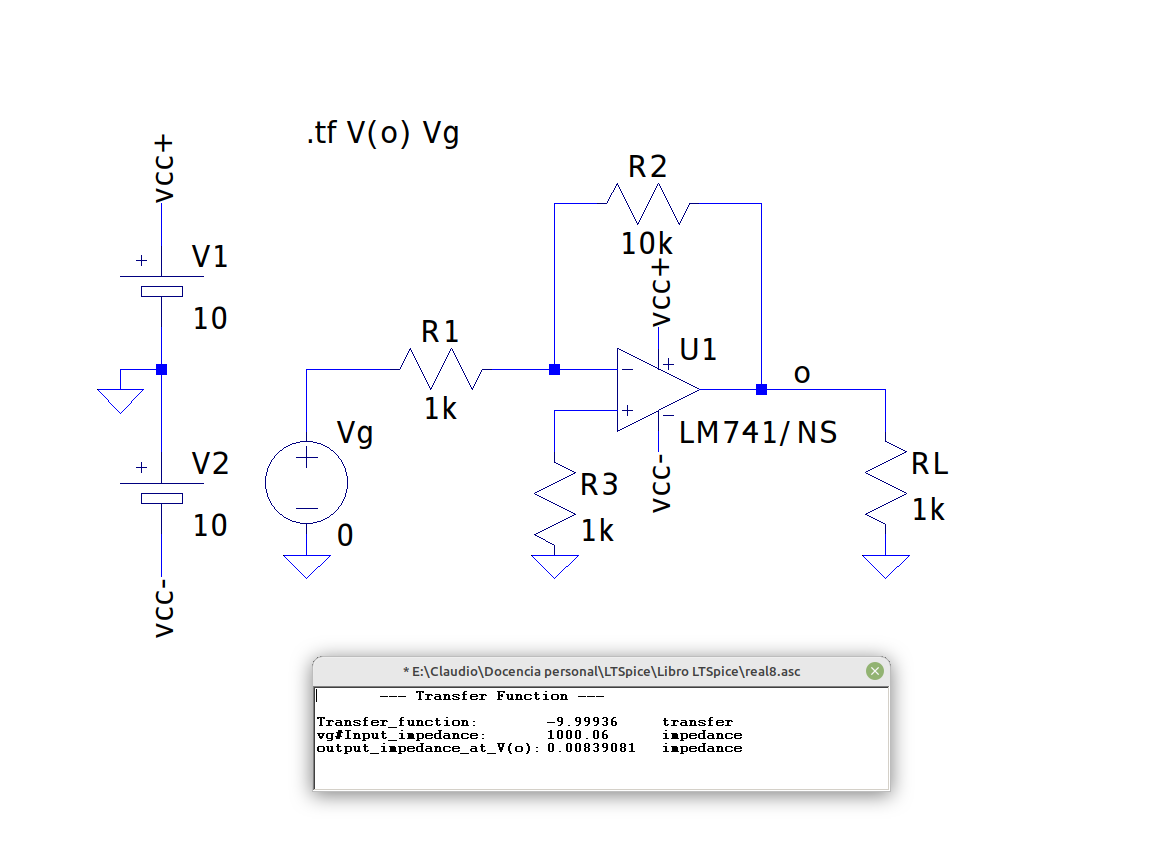
\includegraphics[width=0.8\linewidth]{figuras/real8x.png}
	\caption{Amplificador inversor con Operacional.}
	\label{real8}
\end{figure}

La figura \ref{real9} es un ejemplo de configuración Serie-Serie, en este caso la realimentación tiende a estabilizar la corriente de salida $I(R_5)$, esta se sensa en serie a través de la red compuesta por las resistencias $R_2$, $R_3$ y $R_4$ y se realimenta en serie a la entrada como una tensión proporcional a dicha corriente. En este caso se simula la transferencia por el método de barrido de AC. Del gráfico se extrae $I(R_5)=-38.37868dB$ que es la corriente de salida a una frecuencia de $1KHz$ en la cual la transferencia es plana. Como la entrada se fija unitaria la transferencia es $A_y=\frac{ I(R_5)}{V_g}= 10^{-38.37868/20}=0.001205 \frac{1}{\Omega}$. Si se calcula la transferencia utilizando la directiva \textit{.tf i(vprueba) vg} se obtiene un resultado similar en la transferencia ($0.0120003 \frac{1}{\Omega}$) y se verifica que las impedancias de entrada y salida son muy elevadas.



\begin{figure}[h]
	\centering
	
\includegraphics[width=0.8\linewidth]{figuras/real9.png}
	\caption{Configuración Serie-Serie}
	\label{real9}
\end{figure}
 
 
 \section{Ganancia de lazo}
 
\hspace{10pt} Como se definió en la introducción de este capítulo, la ganancia de lazo $T=a\textsf{f}$ es una cantidad muy importante que caracteriza al amplificador realimentado. También, como se verá en el capítulo siguiente, es de crucial importancia en la determinación de la estabilidad del sistema. En los sistemas lineales, la ganancia de lazo no depende de las entradas sino de la topología del circuito en sí, por lo que puede ser determinada sin la presencia de las entradas.  

Si en el esquema teórico de la figura \ref{real1} anulamos la entrada $X_i=0$, "abrimos el lazo" en la conexión entre las salida $X_o$ y la entrada al bloque de realimentación y colocamos una fuente de prueba $X_p$ en la entrada de $\textsf{f}$, se obtiene que: $X_f =\textsf{f}X_p$, $X_e = 0-X_f=-\textsf{f}X_p$, $X_o =aX_e=-a\textsf{f}X_p$ y por lo tanto $T=a\textsf{f}=-\frac{X_o}{X_p}$.

En el esquema teórico es sencillo abrir el lazo, ya que los bloques son unidireccionales e ideales por lo que el mecanismo utilizado para su cálculo no produce errores y puede ser abierto en cualquier parte del lazo. En los casos prácticos hay que tener algunas consideraciones para poder usar este método en forma adecuada.

\begin{figure}
	\centering
	
\includegraphics[width=0.8\linewidth]{figuras/real10.png}
	\caption{a) Amplificador genérico. b) Apertura del lazo en punto $xy$}
	\label{real10}
\end{figure}

En la figura \ref{real10} a) se muestra un esquema de un amplificador realimentado genérico con la fuente de entrada anulada. Se busca un punto en el circuito en donde se conozca fehacientemente la impedancia que presenta, por ejemplo el punto del corte  $xy$, luego se abre el circuito en ese punto, se inserta una fuente de prueba $V_p$ y se carga el otro extremo del corte con la impedancia $Z_p$ que presenta el circuito. En la figura \ref{real10} b) se esquematiza el procedimiento, la ganancia de lazo se obtiene hallando la transferencia $T=a\textsf{f}=-\frac{V_p'}{V_p}$.
   
   
 
Se puede implementar este criterio para la obtención de la ganancia de lazo mediante LTSpice.  Por ejemplo en el circuito de la figura \ref{real9} se busca un punto en donde la impedancia sea elevada, insertando en serie una fuente de tensión de AC con valor de continua nulo, para luego hacer un barrido de AC y así obtener la transferencia de la ganancia de lazo. En el la figura \ref{real11} se muestran como insertar la fuente y en la figura \ref{real12} los resultados de la transferencia $T=-\frac{V_2}{V_1}$, es de notar que la fuente de prueba se insertó en la entrada positiva del operacional en donde la impedancia de entrada es elevada. Utilizando los modelos de pequeña señal de los dispositivoss se puede verificar que los resultados entre lo simulado y lo teórico son similares.

\begin{figure}
	\centering
	
\includegraphics[width=0.8\linewidth]{figuras/real11.png}
	\caption{Insersión de la fuente de prueba.}
	\label{real11}
\end{figure}

\begin{figure}
	\centering
	
\includegraphics[width=1.0\linewidth]{figuras/real12.png}
	\caption{Diagrama de Bode de la transferencia $T=a\textsf{f}$.}
	\label{real12}
\end{figure}

Otra posibilidad es buscar un punto en donde el circuito actúe como una fuente de tensión aproxi\-ma\-da\-men\-te ideal, en la figura \ref{real11} ese lugar podría ser la salida del operacional, si allí insertamos una fuente de AC del mismo modo que en el caso anterior y realizamos el mismo análisis se verifica que se obtienen resultados similares. Por ejemplo en el primer caso la ganancia de lazo a frecuencias bajas es de $100.63353dB$ y en el segundo $100.66259dB$. 

Si no se pueden encontrar en el circuito puntos de las características presentadas anteriormente se puede utilizar el método propuesto por Rosenstark \cite{Rosenstark86} y desarrollado en \cite{sedra99} para obtener la ganancia de lazo. Tal método se esquematiza en la figura \ref{real13} y consiste en elegir un punto apropiado del circuito, abrir el lazo y obtener la ganancia de circuito abierto $T_{ca}=\frac{V_{ca}}{V_p}$ (figura \ref{real13} a) y la ganancia de corto circuito $T_{cc}=\frac{I_{cc}}{I_p}$ (figura \ref{real13} b). Luego se obtiene la ganancia de lazo como:

\begin{equation}\label{eqros}
	T=\frac{\displaystyle -1}{\displaystyle \frac{\displaystyle 1}{\displaystyle T_{ca}}+\frac{\displaystyle 1}{\displaystyle T_{cc}}}	
\end{equation}.

\begin{figure}
	\centering
	
\includegraphics[width=0.8\linewidth]{figuras/real13.png}
	\caption{Obtensión de $T=a\textsf{f}$ por método de Rosenstark.}
	\label{real13}
\end{figure}


En la figura \ref{real14} se muestra una implementación del método de Rosenstark en LTSpice. Se toma como base el circuito de la figura \ref{real9}, se abre el circuito en la conexión entre $R_3$ y $R_4$ y se hacen dos intervenciones. El circuito de la izquierda representa el cálculo de la transferencia a circuito abierto, como fuente de prueba se coloca en el punto $X_1$ una fuente de tensión de AC de 1V y 0V de continua en serie con un capacitor $C_1$ de un valor teórico muy alto (1F) para que no afecte ni la respuesta en frecuencia ni el punto de continua, además se conecta la realimentación al punto $X_2$ a través de una inductancia teórica muy elevada ($L_1=1gH$) para aislar en alterna el circuito pero no alterar el punto de continua, bajo estas consideraciones se calcula la transferencia de tensión de circuito abierto $T_{ca}=\frac{V(X_2)}{V(X_1)}$. En el circuito de la derecha se coloca una fuente de corriente $I_p$ de AC de 1A y 0A de continua en el punto de inserción, se conecta la realimentación a través de una inductancia $L_2$ de elevado valor para separar en alterna y se conecta una fuente de tensión $V_6=0$, a través de un capacitor $C_2=1F$ para simular el corto circuito, en estas condiciones se obtiene la transferencia de corriente de corto circuito $T_{cc}=\frac{I(V_6)}{I(I_1)}$.
Si hace un barrido de AC a ambos circuitos y se obtienen las transferencias de circuito abierto y corto circuito a una frecuencia donde la transferencia es plana, se puede obtener mediante la ecuación \ref{eqros} el valor de $T=107498.25$ ($100.63dB$) a dicha frecuencia, que es muy similar al obtenido anteriormente por el otro método descripto.

\begin{figure}
	\centering
	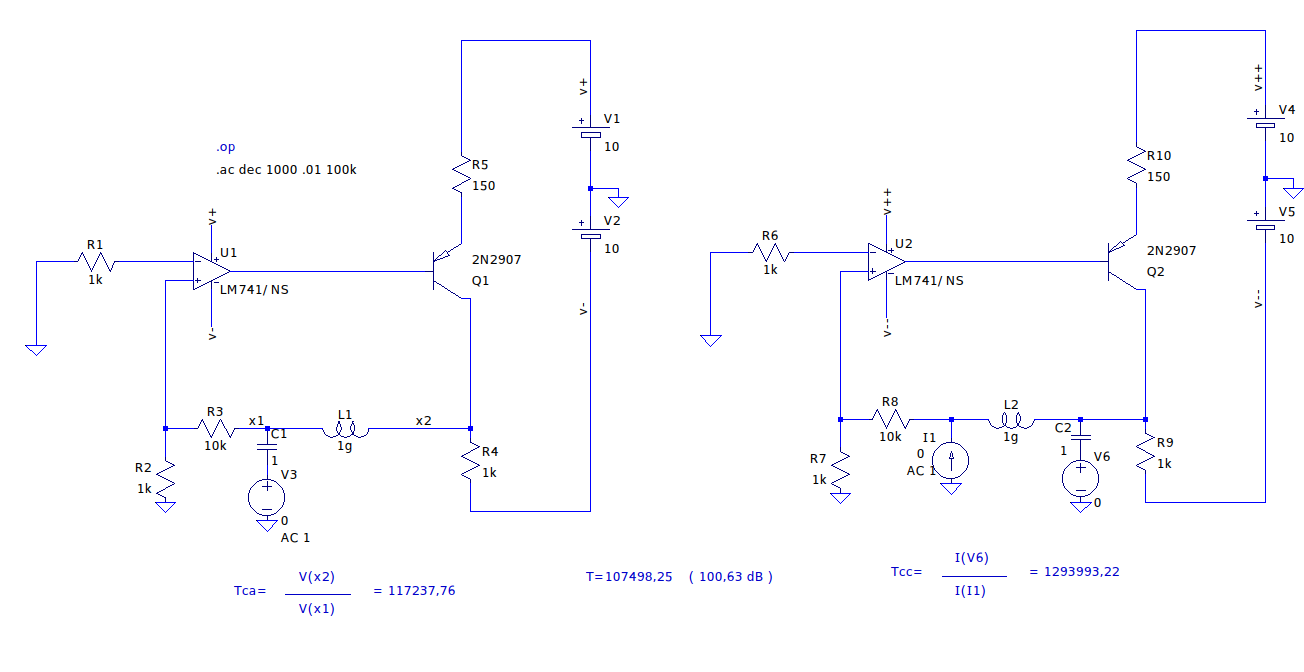
\includegraphics[width=1.0\linewidth]{figuras/real14.png}
	\caption{Método de Rosenstark utilizando LTspice.}
	\label{real14}
\end{figure}
